\chapter{Theoretical Background}
\label{sec:theoretical_background}


\section{Molecular Dynamics}

Molecular Dynamics (MD) is a computational method used to simulate the behavior of atoms and molecules over time. In recent years, MD simulations have become essential in many scientific fields, including chemistry, physics, biology, and materials science. Such simulations are used to study various systems, ranging from simple gases and liquids to complex biological molecules and new materials.

MD simulations act on an atomic level and attempt to explain macroscopic properties of a system from the interactions between the individual atoms and molecules. The recent advances in computational power have made it possible to simulate systems with millions of particles over long time scales, allowing researchers to study complex systems in unprecedented detail. Contrary to experimental methods, MD simulations can provide detailed information about the behavior of atoms and molecules, sometimes inaccessible to experimental methods~\cite{Perilla2017}.

Two illustrations of such simulations are shown in \autoref{fig:hiv_capsid} and \autoref{fig:md_simulation_loop}. The first image shows a simulation of the HIV-1 capsid, a protein shell that surrounds the genetic material of the human immunodeficiency virus (HIV). Using a simulation-based approach, researchers could study critical properties of the HIV-1 capsid, which would be difficult to access using other methods~\cite{Perilla2017}. The second image shows a simulation of shear band formation around a precipitate in metallic glass. This simulation found evidence that depending on the precipitate size, shear bands can either dissolve, wrap around, or be blocked by the precipitate~\cite{Brink2016}. This information is crucial for understanding the mechanical properties of metallic glasses and can be used to design new materials with improved properties.


\begin{multicols*}{2}
      \begin{figure}[H]
            \centering
            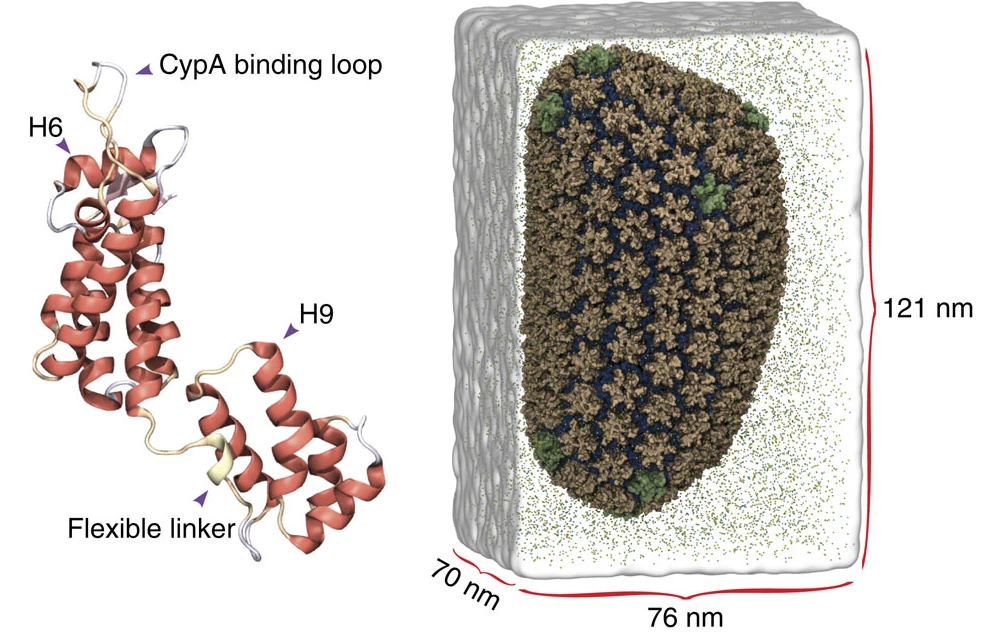
\includegraphics[width=0.9\columnwidth, trim={0cm 0 0cm 0cm}]{figures/Intro/HIV-1.png}
            \caption{MD simulation with 64,423,983 atoms of the HIV-1 capsid. Perilla et al.~\cite{Perilla2017} investigated properties of the HIV-1 capsid at an atomic resolution.}
            \label{fig:hiv_capsid}
      \end{figure}

      \begin{figure}[H]
            \centering
            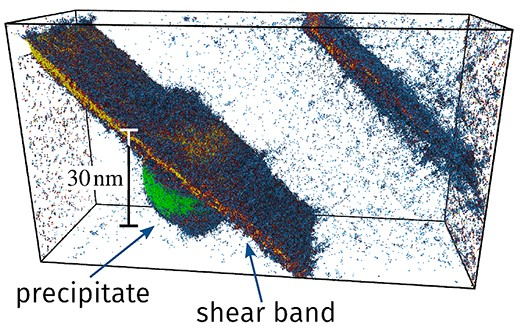
\includegraphics[width=0.9\columnwidth,trim={0cm 0 0cm 0cm}]{figures/Intro/metallic-glass-crack.jpg}
            \caption{MD simulations of shear band formation around a precipitate in metallic glass, as demonstrated by Brink et al.~\cite{Brink2016}.}
            \label{fig:md_simulation_loop}
      \end{figure}
\end{multicols*}

\subsection{Quantum Mechanial Background}

Our current knowledge of physics suggests that the behavior of atoms and molecules is governed by the laws of quantum mechanics, where particles are described by probabilistic wave functions evolving over time. In 1926, Austrian physicist Erwin Schrödinger formulated a mathematical model describing this concept, which has since gained widespread acceptance and is now generally known as the Schrödinger equation. The Schrödinger equation is a partial differential equation describing the time evolution of a quantum system and is given by:

\begin{equation}
      i \hbar \frac{\partial \Psi(\vec{r}, t)}{\partial t} = \hat{H} \Psi(\vec{r}, t)
\end{equation}

Where $\Psi(\vec{r}, t)$ is the system's wave function, evolving over time $t$ and space $\vec{r}$. $\hat{H}$ is the Hamiltonian operator describing the system's energy, $t$ is the time, and $\hbar$ is the reduced Planck constant.
\smallskip

The Schrödinger equation provides a way to calculate the future states of a quantum system given the system's current state. However, the computational complexity of solving this equation increases dramatically with the number of particles involved and quickly becomes infeasible for systems with more than a few particles~\cite{Leimkuhler2015}. To illustrate this complexity, consider simulating a single water molecule. This molecule consists of three nuclei (two hydrogen atoms and one oxygen atom) and 10 electrons. Each of these 13 objects requires three spatial coordinates to describe its position, resulting in a total of $(2+1+10) \times 3 = 39$ variables. The Schrodinger equation for this single water molecule can therefore be written as:

\begin{equation}
      i \hbar \frac{\partial \Psi}{\partial t} = -\hbar^2 \sum_{i=1}^{13} \frac{1}{2m_i} \left( \frac{\partial^2 \Psi}{\partial x_i^2} + \frac{\partial^2 \Psi}{\partial y_i^2} + \frac{\partial^2 \Psi}{\partial z_i^2} \right) + U_p (x_1, y_1, z_1, \ldots, x_{13}, y_{13}, z_{13}) \Psi
\end{equation}

In this equation, $m_i$ is the mass of the $i$-th object, $x_i$, $y_i$, and $z_i$ are the spatial coordinates of the $i$-th object, and $U_p$ is the potential energy function of the system.
\smallskip

As the Schrödinger equation is a partial differential equation, it is computationally expensive to solve for systems with many particles, as one quickly runs into the curse of dimensionality. Larger systems, such as the HIV-1 capsid shown in \autoref{fig:hiv_capsid} consisting of millions of atoms, are practically impossible to simulate using the Schrödinger equation directly.

Luckily, the Born-Oppenheimer approximation simplifies the Schrödinger equation so that it becomes computationally feasible to simulate even large systems of particles. The approximation exploits the significant mass difference between electrons and nuclei\footnote{
      The mass ratio of a single proton to an electron is approximately 1836:1, illustrating the vast difference in mass between nuclei and electrons.
}, making it possible to solve both motions independently~\cite{Zielinski2013}. As the forces acting on the heavy nuclei cause way slower movements compared to the same force acting on the electrons, it is possible to approximate the position of the nucleus as entirely stationary. This simplification yields a new potential energy function $U$ combining all electronic and nuclear energies, which depends only on the nuclei's positions.
The potential energy function $U$ fundamentally controls the motions of the nuclei~\cite{Zielinski2013} and is typically obtained through quantum mechanical calculations or fitted to empirical data~\cite{Irikura2021}.

As the Born-Oppenheimer approximation is based on simplifications of the full model, it is not always accurate. Depending on the system under investigation and the chosen potential energy function $U$, the Born-Oppenheimer approximation may neglect specific quantum mechanical effects, resulting in inaccuracies in the simulation.

Despite these limitations, the Born-Oppenheimer approximation is widely used in molecular dynamics simulations and is the best-known method to simulate systems with many particles.

\subsection{Classical Molecular Dynamics}

After applying the Born-Oppenheimer approximation and using Newton's second law of motion, the Schrödinger equation can be transformed into a system of ordinary differential equations of the form:

\begin{equation}
      m_i \frac{d^2 \vec{r}_i}{dt^2} = -\nabla_i U
\end{equation}

Where $m_i$ is the mass of the $i$-th particle, $\vec{r}_i$ is the position of the $i$-th particle, and $U$ is the potential energy function of the system. These equations precisely describe a classical particle system, where particles are treated as point masses moving through space under the influence of forces. The forces are derived from the potential energy function $U$ and are calculated using the negative gradient of the potential energy function $\nabla_i U$.

\subsection{Potential Energy Function}

As stated above, the potential energy function $U$ is a critical component of molecular dynamics simulations as it fundamentally defines the properties of the system. MD simulations use many different potential energy functions, all of which are tailored to describe specific aspects of the system. Those potentials typically use a mixture of 2-body, 3-body, and 4-body interactions between the particles, each used to describe different aspects of particle interactions. The 2-body interactions typically express the effect of Pauli repulsion, atomic bonds, and coulomb interactions, while higher-order interactions allow for asymmetric wave functions for atoms in bound-groups \cite{Leimkuhler2015}.

A common choice for the potential energy function is the Lennard-Jones potential. This potential can reproduce the potential energy surfaces of many biological systems~\cite{NexusPhysicsLennardJones} while still being very simple and efficient to compute. It mainly emulates the attractive Van-der-Waals forces and the repulsive Pauli repulsion forces between the particles~\cite{ChemieLexikonLennardJones}.

The Lennard-Jones potential is given by:

\begin{equation}
      U_{LJ}(r) = 4 \epsilon \left[ \left( \frac{\sigma}{r} \right)^{12} - \left( \frac{\sigma}{r} \right)^6 \right]
\end{equation}


Where $r$ is the distance between the particles, $\epsilon$ is the depth of the potential well, and $\sigma$ is the distance at which the potential is zero. The parameters $\epsilon$ and $\sigma$ can differ for each type of particle interaction and are either determined from theoretical considerations of the material or chosen to match experimental data~\cite{Maghfiroh2020}.


\subsection{Numerical Integration}

Since the simulation domain potentially consists of a vast number of particles all interacting with each other, it is generally not possible to solve the equations of motion analytically. This problem is known under the N-body problem, and it can be shown that there are no general solutions for systems with more than two particles. It is, however, possible to approximate solutions of these equations of motion using numerical integration methods. A widely used method for this purpose is the Velocity-Störmer-Verlet algorithm. It is defined as follows:

\begin{align}
      \vec{r}_i(t + \Delta t) & = \vec{r}_i(t) + \Delta t \cdot \vec{v}_i(t) + (\Delta t)^2 \frac{\vec{F}_i(t)}{2m_i} \label{eq:verlet_position} \\
      \vec{F}_i(t + \Delta t) & = -\nabla_i U \label{eq:verlet_force}                                                                            \\
      \vec{v}_i(t + \Delta t) & = \vec{v}_i(t) + \Delta t  \frac{\vec{F}_i(t) + \vec{F}_i(t + \Delta t)}{2m_i} \label{eq:verlet_velocity}
\end{align}

Where $\vec{r}_i(t)$ is the position, $\vec{v}_i(t)$ is the velocity, $\vec{F}_i(t)$ is the force acting on the $i$-th particle at time $t$. $\Delta t$ is the time step size, and $m_i$ is the mass of the $i$-th particle. The forces acting on the particles can be calculated from the potential energy function $U$ as $\vec{F}_i(t) = -\nabla_i U$.

\subsection{Simulation Loop}

Using the methods described above, it is possible to simulate the behavior of a system of particles over time. The general simulation loop for a molecular dynamics simulation can be described as follows:


\begin{algorithm}
      \SetAlgoLined
      \textbf{Initialize} particle positions and velocities based on initial conditions\;
      \vspace{0.2cm}
      \While{simulation time $<$ desired time}{
            Update all particle positions using \autoref{eq:verlet_position}\;
            Calculate all forces $\vec{F}_i(t+\Delta t)$ at the new positions using \autoref{eq:verlet_force}\;
            Update all particle velocities using \autoref{eq:verlet_velocity}\;
            \vspace{0.2cm}
            Apply external forces or constraints (if any)\;
            Increment simulation time\;
      }
      \caption{Molecular Dynamics Simulation Loop (Velocity-Störmer-Verlet)}
\end{algorithm}


Many different software packages exist to perform such simulations. Some widely used examples of such systems are LAAMPS\footnote{\url{https://lammps.sandia.gov/}} and GROMACS\footnote{\url{https://www.gromacs.org/}}. Both attempt to efficiently solve the underlying N-body problem and provide the user with a high-level interface to specify the parameters and properties of the simulation.

Many different approaches exist to efficiently solve the N-body problem, and no single best approach works well for all systems as the optimal implementation heavily depends on the simulation state and the hardware used to perform the simulation. However, LAAMPS and GROMACS use a single implementation and cannot adapt their algorithms to the current simulation state.

In the following section, we will introduce AutoPas, a library designed to efficiently deal with evolving particle simulations, leveraging the idea of automatically switching between different implementations to achieve the best performance for the current simulation state.

\section{AutoPas}

AutoPas is an open-source library designed to achieve optimal node-level performance for short-range particle simulations. On a high level, AutoPas can be seen as a black box performing arbitrary N-body simulations with short-range particle interactions. However, AutoPas differentiates itself from other libraries by providing many algorithmic implementations for the N-body problem, each with different performance and memory usage trade-offs. No implementation is optimal for all simulation scenarios, and the optimum can even change during the course of the simulation~\autoref{GRATL2022108262}. Consequently, AutoPas is designed to be adaptive and can periodically switch between different implementations to remain reasonably close to the current optimal configuration.

Since AutoPas provides a high-level interface for short-range N-body simulations, the user must specify the desired model and simulation parameters. Fortunately, AutoPas also provides some example implementations, such as \texttt{\gls{mdflexible}}. \texttt{\gls{mdflexible}} is a simple molecular dynamics framework built on top of AutoPas that allows users to specify the desired simulation parameters and run simulations. This work will primarily focus on \texttt{\gls{mdflexible}}, but the concepts can be easily transferred to other simulation frameworks.

\subsection{Autotuning in AutoPas}

AutoPas internally alternates between two phases of operation. The first phase is the \emph{tuning phase}, where AutoPas tries to find the best configuration of parameters that minimize a chosen performance metric (e.g., time, energy usage) for the current simulation state. This is achieved by trying out different configurations of parameters and measuring their performance. The configuration that optimizes the chosen performance metric is then used in the following \emph{simulation phase}, assuming that the optimal configuration found in the tuning phase still performs reasonably well.
As the simulation progresses and the characteristics of the system change, the previously chosen configuration can drift arbitrarily far from the actual optimal configuration. To counteract this, AutoPas periodically alternates between tuning and simulation phases to ensure that the used configuration remains close to optimal.

The power of AutoPas comes from its vast amount of tunable parameters and the enormous search space associated with them. In the following sections, we will discuss all currently tunable parameters in AutoPas and briefly introduce the different tuning strategies used to guide the search for the best configuration of parameters.

\subsection{Tunable Parameters}

AutoPas currently provides six tunable parameters, which can mostly\footnote{There are some exceptions as some choices of parameters are incompatible with each other.} be combined freely. A collection of parameters is called a \emph{Configuration}, and the set of all possible configurations is called the \emph{Search Space}. Each configuration consists of the following parameters:

\begin{enumerate}[label=\textbf{\arabic*.}]
      \item \textbf{Container Options:} \\
            The container options are related to the data structure used to store the particles. The most important categories of data structures in this section are:
            \begin{enumerate}
                  \item \textbf{DirectSum} \\
                        DirectSum does not use any additional data structures to store the particles. Instead, it simply holds a list of all particles. Consequently, it needs to rely on brute-force calculations of the forces between all pairs of particles. This results in a complexity of $O(N^2)$ distance checks in each iteration. This inferior complexity renders it completely useless for larger simulations.\\
                        \textit{Generally should not be used except for tiny systems or demonstration purposes.~\cite{VICCIONE2008625}}
                  \item \textbf{LinkedCells} \\
                        LinkedCells segments the domain into a regular cell grid and only considers interactions between particles from neighboring cells. This results in the trade-off that particles further away are not considered for the force calculation. In practice, this is not a big issue, as all short-range forces drop off quickly with distance anyway.
                        LinkedCells also provides a high cache hit rate as particles inside the same cell can be stored contiguously in memory. Typically, the cell size is chosen to equal the force cutoff radius $r_c$, meaning each particle only needs to check interactions between particles inside the $3\times3\times3$ cell grid around the current cell. All other particles are guaranteed to be further away than the cutoff radius and, therefore, cannot contribute to the acting forces.
                        This reduction in possible interactions can result in a complexity of just $O(N)$ distance checks in each iteration if the particles are spread evenly. However, there is room for improvement as the constant overhead factor can be pretty high, as most distance checks performed by LinkedCells still do not contribute to the force calculation when using $r_{cell}=r_c$ ~\cite{GRATL2019748}.\\
                        \textit{However, still generally good for large, homogeneous\footnote{Homogeneous in this context, the particles are distributed evenly across the domain.} systems.}

                  \item \textbf{VerletLists} \\
                        VerletLists are another approach to creating neighbor lists for the particles. Contrary to LinkedCells, VerletLists does not rely on a regular grid but instead uses a spherical region around each particle to determine its relevant neighbors. The algorithm creates and maintains a list of all particles present in a sphere within radius $r_c \cdot s$ around each particle, where $r_c$ is the cutoff radius and $s>1$ is the skin factor allowing for a buffer zone around the cutoff radius.
                        By choosing a suitable buffer zone, such that no fast-moving particle can enter the cutoff radius unnoticed, it is possible to only recalculate the neighbor list every few iterations. This method also results in a complexity of $O(N)$ distance checks in each iteration but provides a higher interaction rate between particles of $1/s^3$. Ideally, the skin factor should be chosen so the ratio is close to 1, resulting in no unnecessary distance checks. This, however, reduces the buffer zone around the cutoff radius, meaning that the neighbor list needs to be updated more frequently, or the simulation needs to be run at higher temporal precision to remain accurate. Finding a good balance between the two is therefore of great importance.\\
                        \textit{Generally good for large systems with high particle density.}

                  \item \textbf{VerletClusterLists} \\
                        VerletClusterLists differ from regular VerletLists in the way the neighbor lists are stored. Instead of storing the neighbor list for each particle separately, $n_{cluster}$ particles are grouped into a so-called \emph{cluster}, and a single neighbor list is created for each cluster. This reduces memory overhead as the neighbor list only needs to be stored once for each cluster. Whenever two clusters are close, all interactions between the particles in the two clusters are calculated. This also results in a complexity of $O(N)$ distance checks in each iteration but provides the advantage of greatly reduced memory usage compared to regular VerletLists.\\
                        \textit{Generally suitable for large systems with high particle density}

            \end{enumerate}

            \begin{figure}[H]
                  \centering
                  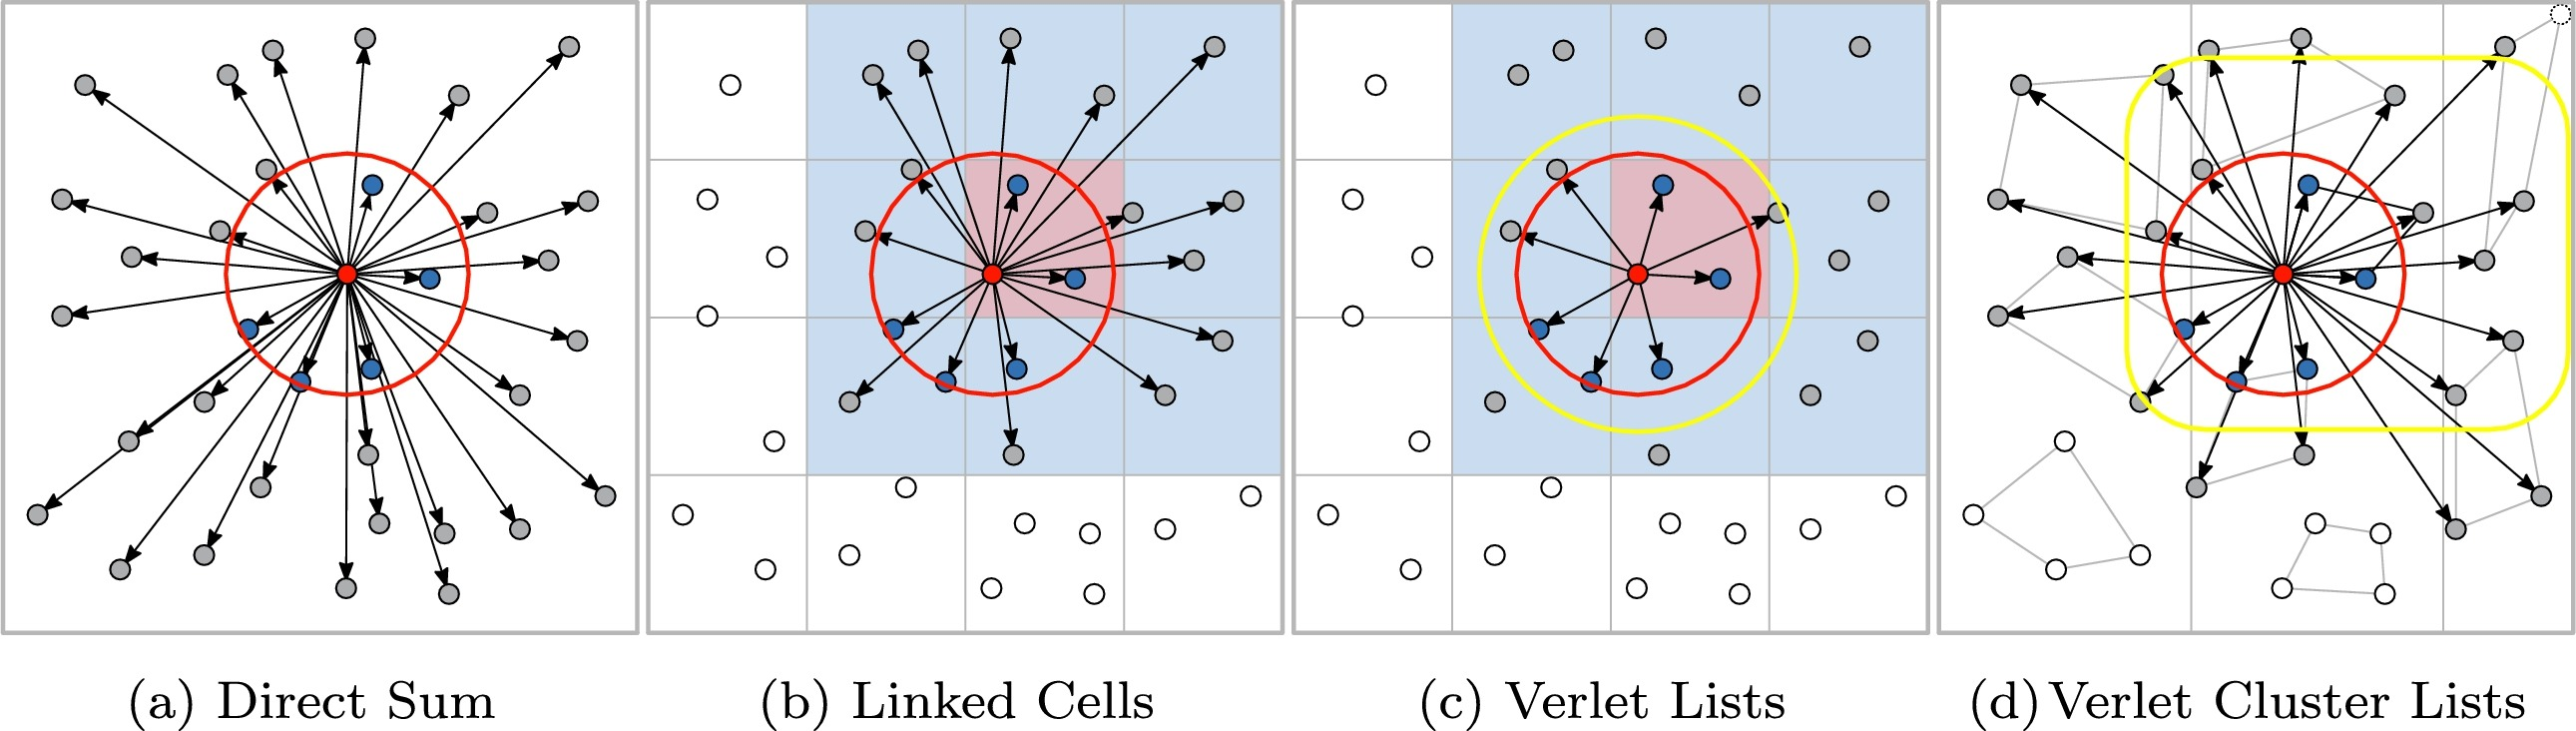
\includegraphics[width=0.9\columnwidth]{figures/Intro/containers.jpg}
                  \caption{Visualization of different container options. \small{Source: Gratl et al.~\cite{GRATL2022108262}}}
                  \label{fig:containers}
            \end{figure}

      \item \textbf{Load Estimator Options:} \\
            The Load Estimator Options relate to how the simulation behaves in a parallelized setting. The load estimator estimates each MPI rank's computational load and guides the simulation's load balancing. In this thesis, however, we will not further describe the Load Estimator Options as we primarily focus on the tuning aspect of single-node simulations.

      \item \textbf{Traversal Options:} \\
            These options are related to the traversal algorithm used to calculate the forces between the particles. The traversal determines the order in which the particles are visited and how the forces are applied to the particles. Furthermore, traversal options should prevent race conditions when using multiple threads and can automatically provide static or dynamic load balancing at the node level~\cite{SECKLER2021101296}.

            Some avaialble traversal options are:

            \begin{enumerate}

                  \item \textbf{Sliced Traversal} \\
                        Sliced Traversal is a way to parallelize the force calculation by dividing the domain into different slices and assigning each to a different thread. When the slices are chosen correctly, no two threads can work on cells with common neighbors, allowing for the force calculation to be parallelized easily, even when using Newton's third law. However, on boundaries, the threads need to be synchronized using locks~\cite{GRATL2022108262} to prevent data races.

                  \item \textbf{Colored Traversal} \\
                        Since both LinkedCells and VerletLists only consider interactions with particles from neighboring cells/particles, it is possible to parallelize the force calculation by calculating forces for particles in different cells in parallel. However, when using Newton's third law, this is only possible if all simultaneously calculated particles do not share familiar neighbors, as updating familiar neighbors could introduce data races when multiple threads act simultaneously. This is where the concept of coloring comes into play. Coloring is a way to assign a color to each cell so that cells with the same color do not share familiar neighbors. This allows for the force calculation of particles in cells with the same color to be parallelized trivially, as data races are impossible. Some ways to color the domain are:
                        \begin{itemize}
                              \item \textbf{C01} \\
                                    The C01 traversal uses no coloring and hands all cells to currently available threads. This method is embarrassingly parallel but comes at the cost of being incompatible with the Newton 3 optimization, as there is no way of preventing data races. As a result, the forces between all pairs of particles are calculated twice, once for each particle. This method results in a constant overhead of factor 2.

                              \item \textbf{C18} \\
                                    The C18 traversal is a more sophisticated way of coloring the domain. The domain is divided into 18 colors, so no two neighboring cells share the same color. This method also utilizes the Newton 3 law to reduce the number of force calculations. This is achieved by only computing the forces with forward neighbors (neighbors with greater index.) ~\cite{GRATL2022108262}

                              \item \textbf{C08} \\
                                    The C08 traversal is closely related to the C18 traversal but only uses eight colors. Due to the fewer colors, there is less synchronization overhead, and a higher degree of parallelism can be achieved. Newton 3 can be used to reduce the number of force calculations
                        \end{itemize}

                        \begin{figure}[H]
                              \centering
                              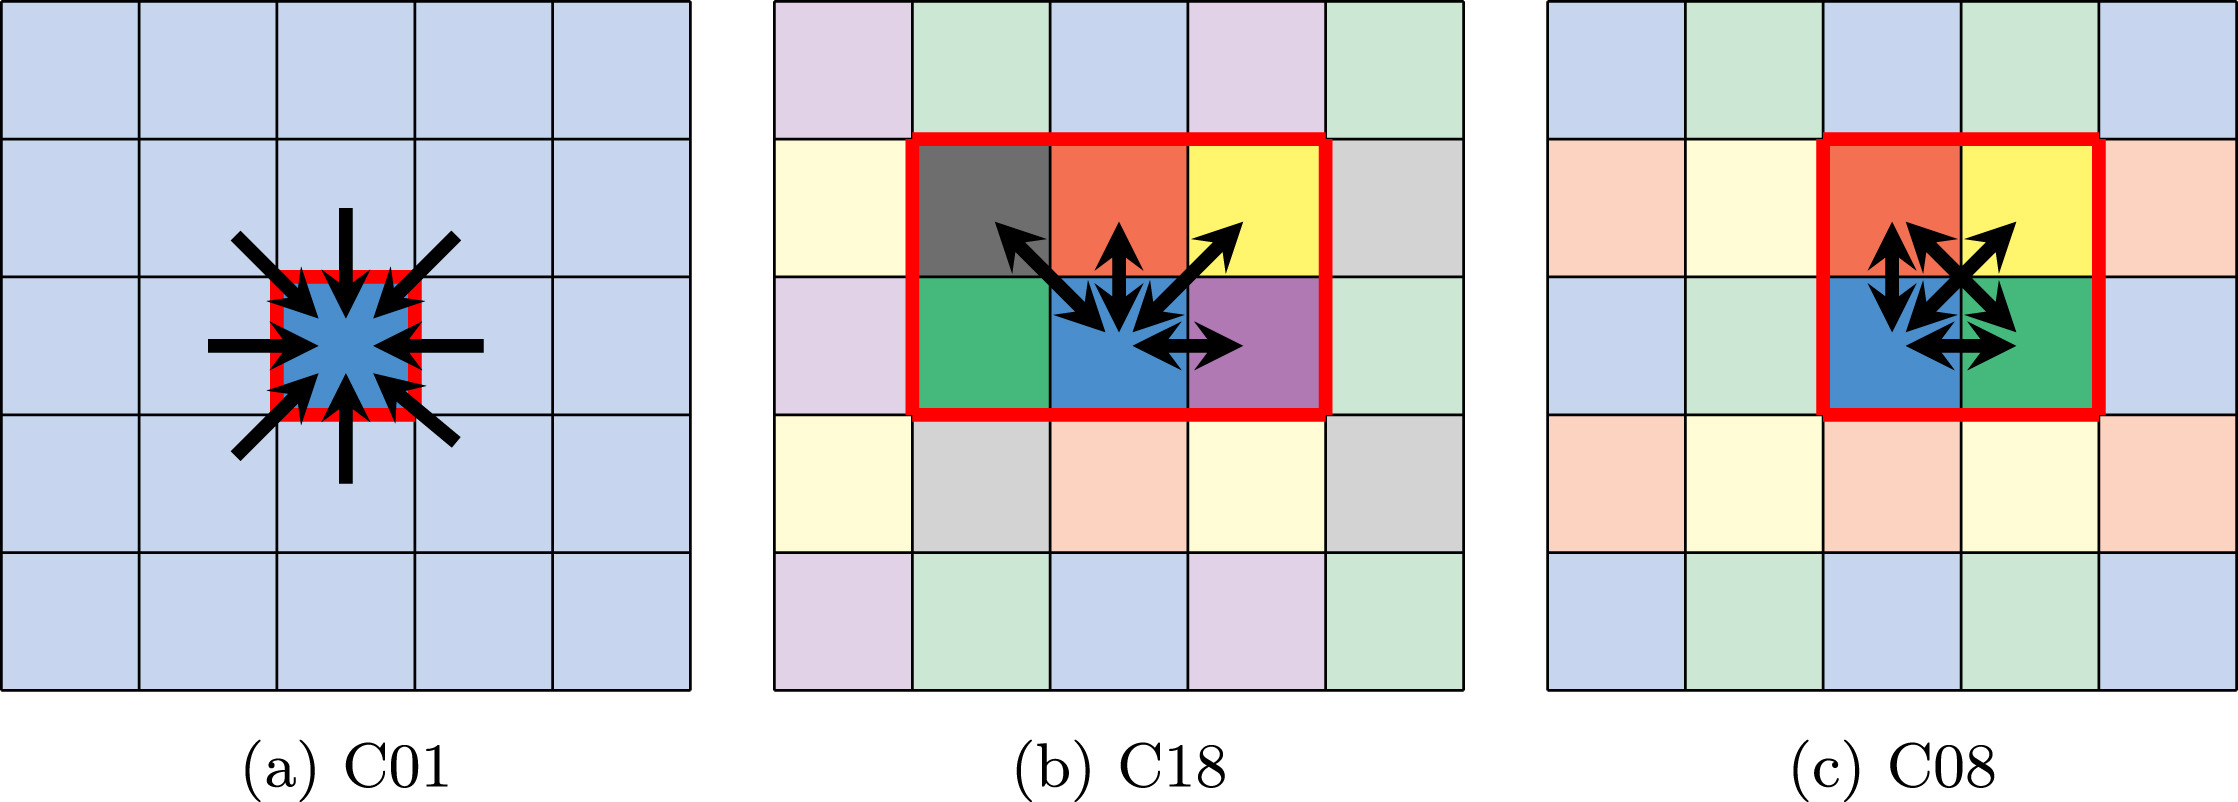
\includegraphics[width=0.7\columnwidth]{figures/Intro/traversals.jpg}
                              \caption{Visualization of different color-based traversal options. \small{Source: Newcome et al.~\cite{Newcome2023}}}
                              \label{fig:traversals}
                        \end{figure}

            \end{enumerate}


      \item \textbf{Data Layout Options:} \\
            The Data Layout Options determine how the particles are stored in memory. The two possible data layouts are:
            \begin{enumerate}
                  \item \textbf{SoA} \\
                        The SoA (Structure of Arrays) data layout stores the particles' properties in separate arrays. For example, all particles' x-,y- and z-coordinates are stored in separate arrays. This data layout is beneficial for vectorization as the properties of the particles are stored contiguously in memory. This allows for efficient vectorization of the force calculations as the properties of the particles can be loaded into vector registers in a single instruction.

                  \item \textbf{AoS} \\
                        The AoS (Array of Structures) data layout stores all particle properties in different structures. This allows for efficient cache utilization when working on particles, as all properties are close to each other in memory. As the same properties of different particles are not stored contiguously, they need to be loaded into vector registers separately, leading to inefficient vectorization.\\
            \end{enumerate}

      \item \textbf{Newton 3 Options:} \\
            The Newton 3 Options relate to how the forces between the particles are calculated. Newton's third law states that for every action, there is an equal and opposite reaction, which means that the magnitude of the force between two particles is the same, regardless of which particle is the source and which is the target. In Molecular Dynamics simulations, this rule can be exploited to reduce the number of force calculations by a factor of 2. The two possible Newton 3 options are:
            \begin{enumerate}
                  \item \textbf{Newton3 Off} \\
                        If Newton 3 is turned off, the forces between all pairs of particles are calculated twice, once for each particle. This results in a constant overhead of factor 2.

                  \item \textbf{Newton3 On} \\
                        If Newton 3 is turned on, the forces between all pairs of particles are calculated only once. There is no more overhead due to recalculating the forces twice, but turning on Newton 3 requires additional bookkeeping, especially in multi-threaded environments. This results in more complicated traversal algorithms and can result in a performance overhead.\\
                        \textit{Generally should be turned on whenever available.}
            \end{enumerate}

      \item \textbf{Cell Size Factor:} \\
            The Cell Size Factor is a parameter that is used to determine the size of the cells in the LinkedCells-Container\footnote{The option is also relevant for other containers such as VerletLists as those configurations internally also build their neighbor lists using a Cell Grid}. If the cell size factor is set to high, many spurious distance checks are performed, as many particles further away than the cutoff radius are considered for the force calculation. Therefore, it is beneficial to reduce the cell size factor. However, the increased overhead of managing more cells can quickly offset the performance gain, and a trade-off between the two needs to be found.\\

\end{enumerate}

\subsection{Tuning Strategies}

Tuning strategies are the heart of AutoPas and attempt to efficiently find the best parameter combination for the current simulation state.

AutoPas provides a couple of different tuning strategies that are used to explore the search space of possible configurations. These tuning strategies aim to quickly find a configuration that minimizes the chosen performance metric. The tuning strategies differ in how they explore the search space and how they decide which configurations to test next.

The currently available tuning strategies in AutoPas are:


\begin{enumerate}
      \item \textbf{Full Search} \\
            The Full Search strategy is the default tuning strategy in AutoPas. It tries out all possible combinations of parameters and chooses the one that optimizes the chosen performance metric. This approach is guaranteed to find the best parameters for the current simulation state. However, it is typically very costly in terms of time and resources as it has to spend a lot of time measuring bad parameter combinations. This is a big issue as the number of possible parameter combinations grows exponentially with the number of parameters, and many of them potentially perform very poorly. This makes the full search approach infeasible, especially if more tunable options are added to AutoPas.

      \item \textbf{Random Search} \\
            The Random Search strategy is a simple tuning strategy that randomly samples a given number of configurations from the search space and chooses the one that optimizes the chosen performance metric. This approach is faster than the Full Search strategy as it does not need to test all possible combinations of parameters. However, it does not guarantee to find the best parameters for the current simulation state.

      \item \textbf{Predictive Tuning} \\
            The Predictive Tuning strategy attempts to extrapolate previous measurements to predict how the configuration would perform in the current simulation state. It filters the search space and only keeps configurations predicted to perform reasonably well. The extrapolations are accomplished using methods such as linear regression or constructing polynomial functions through the data points.

      \item \textbf{Bayesian Search} \\
            Two implementations of Bayesian tuning exist in AutoPas. Those methods apply Bayesian optimization techniques to predict suitable configurations using performance evidence from previous measurements.

      \item \textbf{Rule Based Tuning} \\
            The Rule Based Tuning strategy uses a set of predefined rules to automatically filter out configurations that are expected to perform poorly. The rules are built on expert knowledge and could look like this:
            \begin{small}
                  \begin{verbatim}
            if numParticles < lowNumParticlesThreshold:
                  [dataLayout="AoS"] >= [dataLayout="SoA"] with same 
                        container, newton3, traversal, loadEstimator;
            endif
            \end{verbatim}
            \end{small}
            The rule states that the data layout "AoS" is generally better than "SoA" if the number of particles is below a certain threshold. The rule-based method can be very effective if the rules are well-designed.
\end{enumerate}


This thesis aims to extend these tuning strategies with a new approach based on Fuzzy Logic. Conceptually, this new fuzzy logic-based tuning strategy is very similar to the rule-based tuning strategy as it uses expert knowledge encoded in fuzzy rules to prune the search space. However, contrary to classical rules, fuzzy logic can deal with imprecise and uncertain information, which allows it to only partially activate rules depending on the \emph{degree of truth} of the condition.
All the suggestions can then be combined based on their degree of activation rather than just following the binary true/false logic. This allows for a more nuanced approach and allows the tuning strategy to interpolate the effect of many different rules to choose the best possible configuration, even if there is no direct rule for this specific case.

In the following section, we will introduce the basic fuzzy logic concepts.


\section{Fuzzy Logic}

Fuzzy Logic is a mathematical framework that allows for reasoning under uncertainty. It is an extension of classical logic and extends the concept of binary truth values ($true$ and $false$) to a continuous range of truth values in the interval $[0, 1]$. Instead of just having true or false statements, it is now possible for statements to be, for example, 40\% true. This concept is beneficial when modeling human language, as the words tend to be imprecise. For example, \emph{hot} can mean different things to different people. For some people, a temperature of 30 degrees Celsius might be considered \emph{hot}, while for others, a temperature of 40 degrees Celsius might be considered \emph{hot}. There is no clear boundary between what is considered hot and what is not, but rather a gradual transition between the two. Fuzzy Logic allows modeling such gradual transitions by assigning a degree of truth to each statement.

\subsection{Fuzzy Sets}

Mathematically, the concept of Fuzzy Logic is based on Fuzzy Sets. A Fuzzy Set is a generalization of a classical set where an element can lie somewhere between being a set member and not being a member. Instead of having a binary membership function that assigns a value of 1 to elements that are members of the set and 0 to elements that are not, elements in a fuzzy set have a certain degree of membership in the set. This degree of membership takes values in the interval $[0, 1]$ where $0$ means that the element is not a member of the set, and $1$ means that the element is a full member of the set.

Formally a fuzzy set $\tilde{A}$ over a crisp/classical set $X$ is defined by a membership function
\begin{equation}
      \mu_{\tilde{A}}: X \rightarrow [0, 1]
\end{equation}

which assigns each element $x \in X$ a degree of membership in the interval $[0, 1]$. The classical counterpart of the element operator could be written as $\in_A: X \rightarrow \{true, false\}$.

The shape of the function can be chosen freely and depends on the specific application. However, typical choices involve triangular, gaussian, or sigmoid-shaped functions, depending on whether the value represents one- or two-sided properties.


\begin{figure}[H]
      \centering
      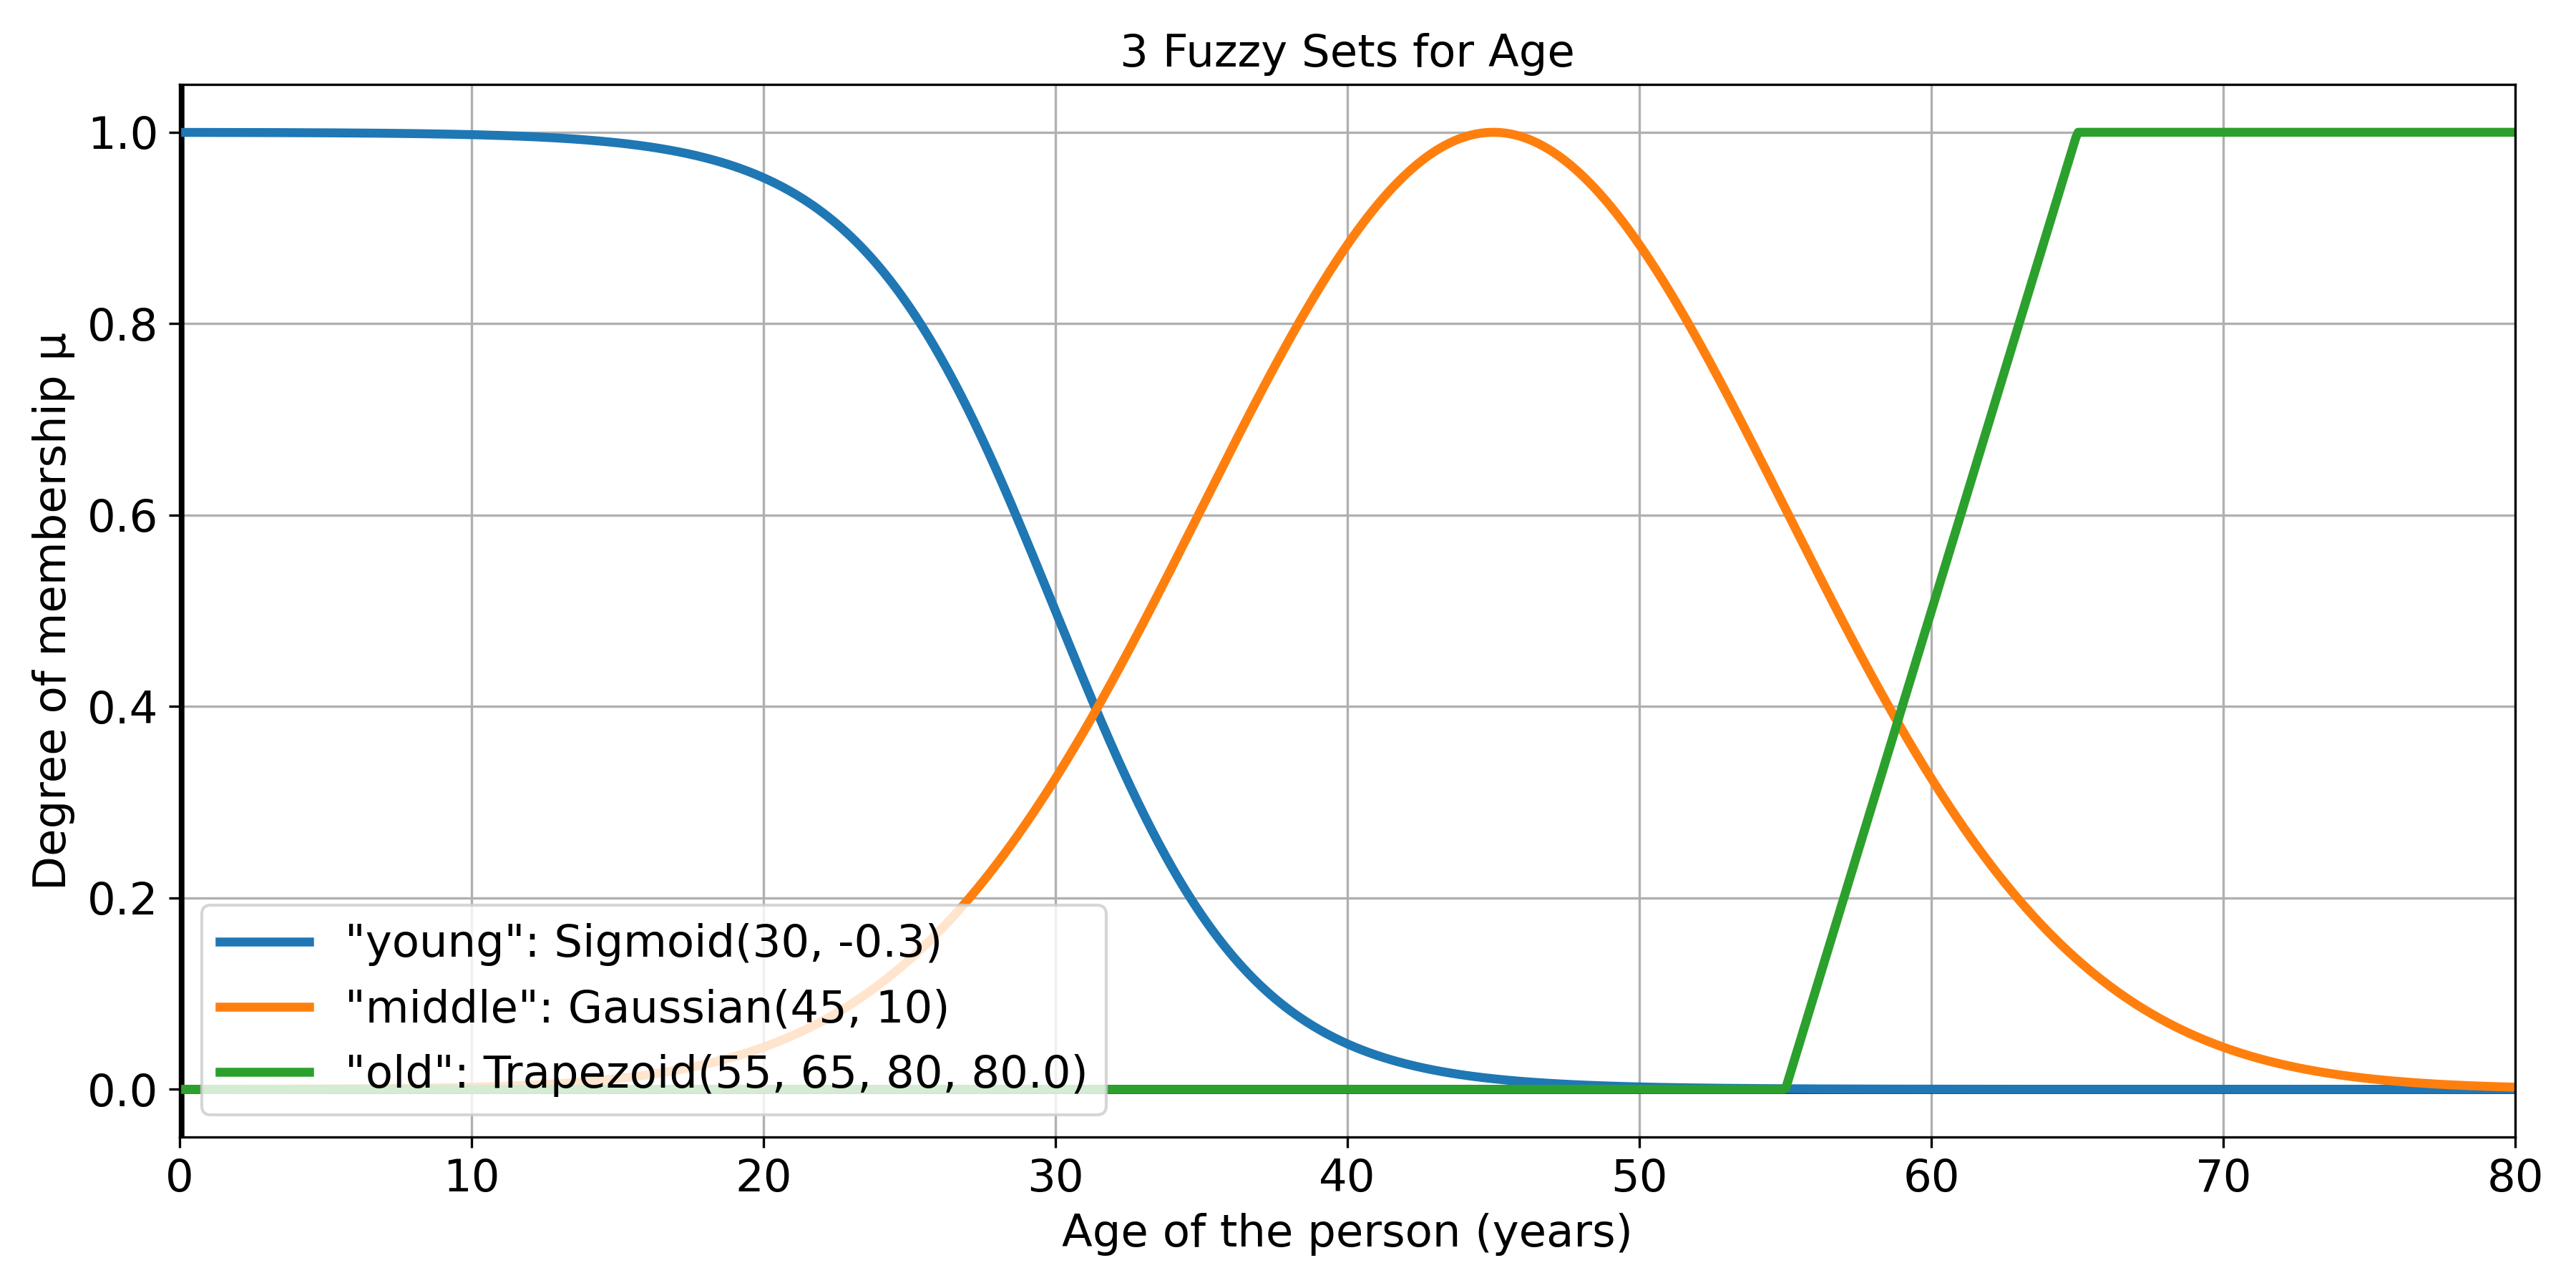
\includegraphics[width=0.8\columnwidth,trim={0 0 0 1cm},clip]{figures/Intro/age-fuzzy-sets.png}
      \caption{Example of fuzzy sets for the age of a person. Fuzzy sets can be used to model the gradual transition between age groups. The distributions could be derived from survey data on how people perceive age groups. In this example, most people would consider a person middle-aged if they are between 35 and 55; there are, however, outliers ranging as low as 20 and as high as 70.}
      \label{fig:fuzzy_sets}
\end{figure}

\subsection{Fuzzy Logic Operations}

Fuzzy Sets are a generalization of classical sets, and as such, they also support the classical set operations of union, intersection, and complement. Those operations need to be extended to work with fuzzy sets and combine both the semantics of classical sets and the concept of vague membership degrees of fuzzy sets.

The extension of classical operators to fuzzy sets uses so-called De Morgan Triplets. Such a triplet $(\top, \bot, \neg)$ consists of a t-norm $\top : [0, 1] \times [0, 1] \rightarrow [0, 1]$, a t-conorm $\bot : [0, 1] \times [0, 1] \rightarrow [0, 1]$ and a strong complement operator $\neg : [0, 1] \rightarrow [0, 1]$. Those operators generalize the classical logical operators, which are only defined on the binary truth values $\{true, false\}$ to continuous values from the continuous interval $[0, 1]$. $\top$ generalizes the logical AND operator, $\bot$ generalizes the logical OR operator, and $\neg$ generalize the logical NOT operator. Instead of the binary functions used in classical logic, those new operators are continuous functions implementing mappings between degrees of truth.

The binary operators $\top$ and $\bot$ are often written in infix notation as $a \; \top \; b$ and $a \; \bot \; b$, similar to how classical logical operators are written.
\smallskip

For the t-norm $\top$ to be valid, it needs to satisfy the following properties:
\begin{align*}
      a \top b          & = b \top a                                                    &  & \text{(Commutativity)}    \\
      a \top b          & \leq c \top d \quad \text{if } a \leq c \text{ and } b \leq d &  & \text{(Monotonicity)}     \\
      a \top (b \top c) & = (a \top b) \top c                                           &  & \text{(Associativity)}    \\
      a \top 1          & = a                                                           &  & \text{(Identity Element)}
\end{align*}

A strong complement operator $\neg$ needs to satisfy the following properties:
\begin{align*}
      \neg 0      & = 1                                   &  & \text{(Boundary Conditions)} \\
      \neg 1      & = 0                                   &  & \text{(Boundary Conditions)} \\
      \neg y      & \leq \neg x \quad \text{if } x \leq y &  & \text{(Monotonicity)}        \\
      \neg \neg x & = x                                   &  & \text{(Involution)}
\end{align*}

The default negation operator in fuzzy logic is $\neg x = 1 - x$. This negation operator satisfies all the abovementioned properties and is the most common choice in practice. In the following sections, we will only consider this standard negation operator.

As in classical logic, the t-conorm $\bot$ can be expressed using $\top$ when applying the generalized De Morgan's laws. De Morgan's laws state that $a \; \lor \; b = \neg(\neg a \; \land \; \neg b)$ for classical logic, which results in $\bot(a, b) = 1 - \top(1 - a, 1 - b)$ for fuzzy logic. Consequently, the properties of the t-conorm can be expressed using the t-norm's properties and omitted here for brevity.


Some common choices for t-norms and t-conorms used in practice are shown in Table~\ref{tab:tnorms}.



\begin{table}[H]
      \centering
      {\renewcommand{\arraystretch}{1.2}
            \begin{tabular}{|c|c|c|c|}
                  \hline
                  Name        & t-norm   $a \top b$                         & Corresponding t-conorm      $a \bot b$ \\
                  \hline
                  Min/Max     & $\min(a, b)$                                & $\max(a, b)$                           \\
                  Algebraic   & $a \cdot b$                                 & $a + b - a \cdot b$                    \\
                  Einstein    & $\frac{a \cdot b}{2 - (a + b - a \cdot b)}$ & $\frac{a + b}{1 + a \cdot b}$          \\
                  Lukasiewicz & $\max(0, a + b - 1)$                        & $\min(1, a + b)$                       \\
                  \hline
            \end{tabular}
      }
      \caption{Common t-Norms and corresponding t-Conorms concerning the standard negation operator $\neg x = 1 - x$}
      \label{tab:tnorms}
\end{table}


With these choices of t-norms, t-conorms, and negation operators, it is possible to define the classical set operations of union, intersection, and complement for fuzzy sets. We will only consider the minimum t-norm and maximum t-conorm in the following sections as they are the most common choices in practice. However, we included a comparison of different t-norms and their effect on the intersection operation in ~\autoref{fig:tnorms}.

\begin{itemize}

      \item \textbf{Intersection} \\
            By expanding the definition of the classical set operation $\cap$ using its boolean form $x \in A \cap B \; \iff \; x \in A \; \land \; x \in B$, we can directly translate this to the fuzzy set intersection operation using the t-norm $\top$. The resulting membership function is given by $\mu_{\tilde{A} \cap \tilde{B}}(x) = \mu_{\tilde{A}}(x) \; \top \; \mu_{\tilde{B}}(x)$. Using the minimum t-norm, the intersection of two fuzzy sets $\tilde{A}$ and $\tilde{B}$ is described by the following membership function:

            \begin{equation*}
                  \mu_{\tilde{A} \cap \tilde{B}}(x) = \min(\mu_{\tilde{A}}(x), \mu_{\tilde{B}}(x))
            \end{equation*}


      \item \textbf{Union} \\
            By expanding the definition of the classical set operation $\cup$ using its boolean form $x \in A \cup B \; \iff \; x \in A \; \lor \; x \in B$, we can directly translate this to the fuzzy set union operation using the t-conorm $\bot$. The resulting membership function is given by $\mu_{\tilde{A} \cup \tilde{B}}(x) = \mu_{\tilde{A}}(x) \;\bot \; \mu_{\tilde{B}}(x)$. Using the maximum t-conorm, the union of two fuzzy sets $\tilde{A}$ and $\tilde{B}$ is described by the following membership function:

            \begin{equation*}
                  \mu_{\tilde{A} \cup \tilde{B}}(x) = \max(\mu_{\tilde{A}}(x), \mu_{\tilde{B}}(x))
            \end{equation*}

      \item \textbf{Complement} \\
            By again expanding the definition of the classical set operation $A^c$ using its boolean form $x \in A^c \; \iff \; \neg (x \in A)$, we can directly translate this to the fuzzy set complement operation using the negation operator $\neg$. The resulting membership function is given by $\mu_{ \tilde{A}^c}(x) = \neg \mu_{\tilde{A}}(x)$. Using the standard negation operator, the complement of a fuzzy set $\tilde{A}$ is described by the following membership function:

            \begin{equation*}
                  \mu_{ \tilde{A}^c}(x) = 1 - \mu_{\tilde{A}}(x)
            \end{equation*}
\end{itemize}


\begin{figure}
      \centering
      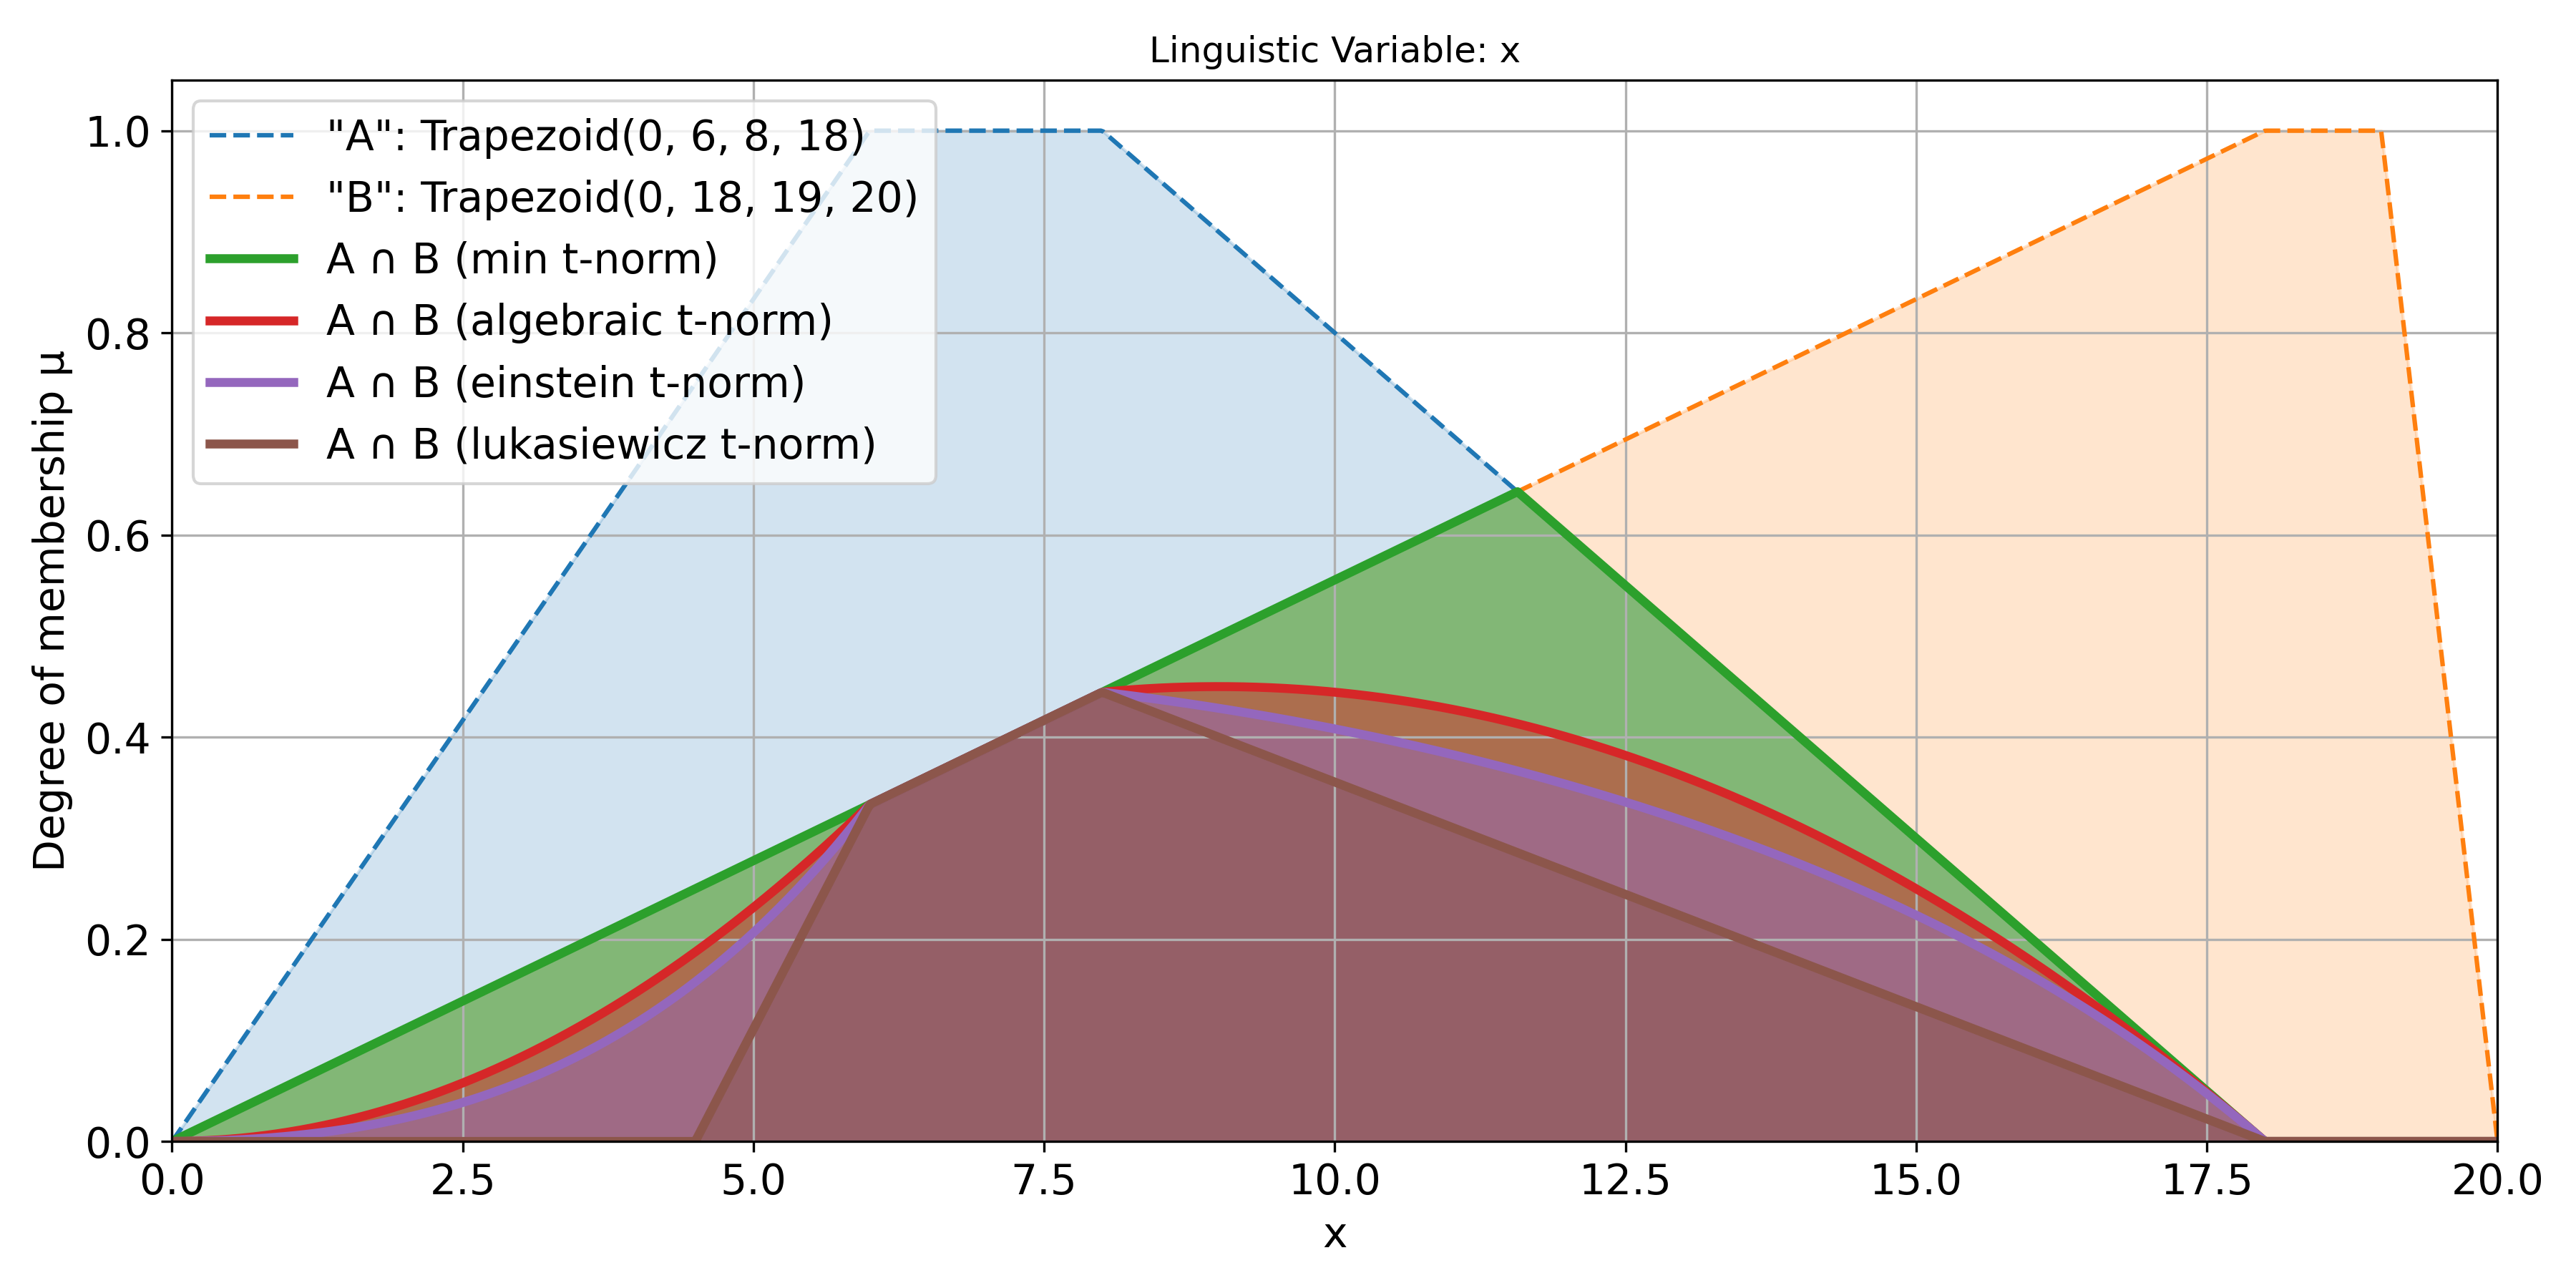
\includegraphics[width=0.9\columnwidth,trim={0 0 0 0.85cm},clip]{figures/Intro/tnorms.png}
      \caption{Effect of different t-norms on the intersection of two fuzzy sets $\tilde{A}$ and $\tilde{B}$. We can see that the choice of t-norm significantly affects the shape of the resulting fuzzy set.}
      \label{fig:tnorms}
\end{figure}


\subsection{Linguistic Variables}

Linguistic variables collect multiple fuzzy sets defined over the same crisp set $X$ into a single object. This variable then allows us to reason about the possible states of the variable more naturally.
Contrary to their classical counterparts, linguistic variables do not take a precise numerical value but rather a vaguely defined linguistic term.
For example, all fuzzy sets depicted in \autoref{fig:fuzzy_sets} form the linguistic variable ``age''. Instead of precisely stating the age of a person using a numerical value, we can now declare the person to be \emph{young}, \emph{middle-aged}, or \emph{old}, where the underlying fuzzy sets capture the transition between those states.


\subsection{Fuzzy Logic Rules}

Fuzzy Logic Rules are a way to encode expert knowledge into a Fuzzy Logic system. The rules specify the relationship between input and output variables of the system and, therefore, are the backbone of fuzzy logic systems.
The rules are typically encoded in a human-readable way and often have the form "$\text{IF} \; \text{antecedent} \; \text{THEN} \; \text{consequent}$" where both the antecedent and the consequent are fuzzy sets. The antecedent is a condition that must be satisfied for the rule to be applied, while the consequent is the action taken if the rule is applied. Since we are not dealing with binary truth values, it is possible that the antecedent is only partially satisfied. As a result, the rule's effect is also only partially considered.

The antecedent can be arbitrarily complicated and may consist of multiple fuzzy sets and logical operators. The consequent is typically a single fuzzy but could theoretically also be arbitrarily complicated. In the implementation of this thesis, we will consider rules generated by the following grammar:

%makro for fuzzy set
\newcommand{\fuzzyset}{\langle \text{fuzzy set} \rangle}

\newcommand{\fuzzyrule}{\langle \text{rule} \rangle}

\begin{align*}
      \text{FuzzyRule} \;::=\; & \text{IF } \text{FuzzySet } \text{THEN } \text{FuzzySet} &  & \text{(Rule)}        \\[10pt]
      \text{FuzzySet} \;::=\;  & \; (\text{FuzzySet})                                     &  & \text{(Parentheses)} \\
                               & | \;\text{FuzzySet } \text{AND } \text{FuzzySet}         &  & \text{(Conjunction)} \\
                               & | \;\text{FuzzySet } \text{OR } \text{FuzzySet}          &  & \text{(Disjunction)} \\
                               & | \;\text{NOT } \text{FuzzySet}                          &  & \text{(Negation)}    \\
                               & | \;\tilde{A} = a                                        &  & \text{(Selection)}
\end{align*}

The boolean operators AND, OR, and NOT represent the set operations of intersection, union, and complement, respectively. The selection operator $\tilde{A} = a$ states that the linguistic variable $\tilde{A}$ should have a high degree of membership in the fuzzy set $a$ for the rule to be activated fully.


Using this grammar, a typical rule might look like this:

\begin{equation*}
      \text{IF} \;( \tilde{A} = a \; \text{AND} \; \tilde{B} = b )\; \text{THEN} \; \tilde{C} = c
\end{equation*}

This rule states that if the state of the linguistic variable $A$ is $a$ and the state of the linguistic variable $B$ is $b$, then the state of the linguistic variable $C$ should be $c$. However, contrary to classical logic, the rule does not have to activate fully but can have a degree of activation in the interval $[0, 1]$.

\smallskip

The inference step can be seen as an extension of the boolean implication operator

\begin{equation*}
      \text{IF} \; \text{antecedent} \; \text{THEN} \; \text{consequent} \iff (\text{antecedent} \implies \text{consequent})
\end{equation*}

Instead of deriving the membership function of the implication operator, the Mamdani implication is typically used. This particular implication is defined as the AND operation $\min(a,b)$. This choice is counterintuitive as it violates its equivalent in classical logic. However, in the context of fuzzy systems, it is a preferred choice, as instead of evaluating the truthiness of the implication, it computes the degree of activation for a rule~\cite{BouchonMeunier1995}.

\subsubsection{Evaluation of Fuzzy Logic Rules}

Consider the rule $\text{IF} \; \tilde{A} = a \; \text{THEN} \; \tilde{C} = c$. To calculate the resulting fuzzy set, we perform the following steps:

\begin{enumerate}
      \item Obtain the input values $(x_1, x_2, \ldots, x_n) \in X_{A}$ occuring in the crisp set of the antecedent.
      \item Evaluate the degree of membership $\mu$ of those input values in the antecedent. This is the degree to which the antecedent is satisfied, and the rule is activated.
      \item Define a new fuzzy set $R=\tilde{C}\uparrow \mu$ as the result of the rule activation. $\uparrow$ is the cut operator and is defined as $\mu_{\tilde{C}\uparrow \mu}(x) = \min(\mu_{\tilde{C}}(x), \mu)$ following the Mamdani implication.
\end{enumerate}

The same steps are performed for every other rule, and the resulting fuzzy sets are combined using the fuzzy union operation specified in the previous section. This final fuzzy set represents the combined effect of all the rules on the output variable.

\subsection{Defuzzification}

The final step in a Fuzzy Logic system is the defuzzification step. In this step, the resulting fuzzy set from the previous section is converted back into a crisp, numeric value that can be used as a concrete output or decision. There are many ways to defuzzify a fuzzy set, but a common theme is finding a representative value that maintains certain aspects of the fuzzy set. In the following sections, we will explore several defuzzification methods:

\begin{itemize}
      \item \textbf{Centroid} \\
            The Centroid method calculates the center of mass of the fuzzy set and returns this value as the crisp output. This method tries to find a weighted interpolation of all the activated fuzzy sets and tries to find an optimal compromise between all the possible values. The Centroid method is the most common defuzzification method and is often used in practice due to its simplicity and robustness. It is defined as:

            \begin{equation}
                  \text{Centroid} = \frac{\int_X x \cdot \mu_{\tilde{C}}(x) \, dx}{\int_X \mu_{\tilde{C}}(x) \, dx}
            \end{equation}

      \item \textbf{Mean of Maximum} \\
            The Mean of Maximum method is simpler than the Centroid method and only considers values, resulting in the highest possible membership value. If multiple such values exist, the arithmetic mean of those values is returned. Contrary to the Centroid method, there is usually no interpolation between the different fuzzy sets, as they usually have different degrees of activation. It is defined as follows:

            \begin{equation}
                  \text{Mean of Maximum} = \frac{\int_{X'} x \, dx}{\int_{X'}  \, dx}
            \end{equation}
            where $X'$ is the set of all input values resulting in the maximum membership value of the fuzzy set.
\end{itemize}
